\documentclass[aspectratio=169]{beamer}

% Packages
\usepackage{amsmath, amssymb, amsthm}
\usepackage{graphicx}
\usepackage{listings}
\usepackage{xcolor}
\usepackage[style=ieee, backend=biber]{biblatex}
\addbibresource{ref.bib}

% Code
\usepackage{listings}
\usepackage{xcolor}
 
% Code style
\lstdefinestyle{Python}{
   language=Python,
    basicstyle=\ttfamily\footnotesize,
    keywordstyle=\color{blue},
    commentstyle=\color{orange},
    stringstyle=\color{red},
    showstringspaces=false,
    breaklines=true,
    breakatwhitespace=true,
    tabsize=2,
    numbers=left,
    numberstyle=\tiny,
    numbersep=5pt,
    frame=single,
    framesep=5pt,
    xleftmargin=15pt,
    xrightmargin=15pt,
    aboveskip=0pt,
    belowskip=0pt,
    backgroundcolor=\color{white}
  }

% Beamer Theme
\usetheme{metropolis}
\usecolortheme{default}

% Title Page
\title{Equilibrium Temperature Distributions using Linear Algebra}
\author{Ali Ehab\and Marwan Basem\and SalahDin Rezk}
\institute{Zewail City - University of Science and Technology}
\date{Fall 2023}

\begin{document}

\begin{frame}
  \titlepage
\end{frame}

\begin{frame}{Outline}
  \tableofcontents
\end{frame}

\section{Introduction}

\begin{frame}{Introduction}
  \begin{itemize}
    \item The heat equation and Laplace's equation \cite{stein}.
    \item Objective: Study equilibrium temperature distributions.
    \item Numerical solutions using Linear Algebra.
  \end{itemize}
\end{frame}

\section{Problem}

\begin{frame}{Problem Statement}
  \begin{itemize}
    \item Given temperature on boundaries of a plate.
    \item Determine temperature inside the plate.
    \item Solve steady-state heat equation ($\Delta u = 0$) numerically.
  \end{itemize}
\end{frame}

\section{Solution}

\begin{frame}{Solution Overview}
  \begin{itemize}
    \item Discretize problem on an $n\times n$ grid.
    \item Apply mean-value property of Laplace's equation \cite{anton}.
    \item Formulate system of linear equations.
    \item Solve numerically using inverse matrix or Jacobi iteration.
  \end{itemize}
\end{frame}

\begin{frame}{Inverse Matrix Method}
  \begin{itemize}
    \item Rewrite system of equations using matrix notation.
    \item Calculate inverse of $(\textbf{\textit{I}} - M)$.
    \item Obtain solution vector $\textbf{t}$.
  \end{itemize}
\end{frame}

\begin{frame}{Jacobi Iteration Method}
  \begin{itemize}
    \item Iteratively update temperature values.
    \item Convergence criteria: $\|\textbf{t}_\text{new} - \textbf{t}\| < \text{tol}$.
    \item Provide initial guess, tolerance, and maximum iterations.
  \end{itemize}
\end{frame}

\section{Implementation}

\begin{frame}{Implementation Details}
  \begin{itemize}
    \item Code implemented in Python using NumPy \cite{gandhi}.
    \item Version control with Git and hosted on GitHub.
    \item Modular code structure for clarity.
  \end{itemize}
\end{frame}

\begin{frame}{Code Structure}
  \begin{itemize}
    \item \texttt{main.py}: Main script for running the program.
    \item \texttt{matrix\_solvers.py}: Functions for solving the system of equations.
    \item \texttt{temperature\_solver.py}: Functions for solving the heat equation.
    \item \texttt{plotting.py}: Functions for plotting the results.
  \end{itemize}
\end{frame}

\begin{frame}[fragile]{Importing libraries}
\begin{lstlisting}[style=Python]
import numpy as np
import matplotlib.pyplot as plt
from mpl_toolkits.mplot3d import Axes3D
\end{lstlisting}
\end{frame}


\begin{frame}[fragile]{Matrix Solvers}
\begin{lstlisting}[style=Python]
def calculate_inverse_solution(A, b):
    A_inverse = np.linalg.inv(A)
    x = np.dot(A_inverse, b)
    return x
\end{lstlisting}
\end{frame}

\begin{frame}[fragile]
\begin{lstlisting}[style=Python]
def jacobi_iteration(A, b, x0=None, tol=1e-6, max_iter=1000):
    n = len(b)
    x = x0 if x0 is not None else np.zeros(n)
    z_iter = np.zeros((max_iter, n))

    for k in range(max_iter):
        x_new = np.zeros_like(x)

        for i in range(n):
            sigma = np.dot(A[i, :i], x[:i]) + np.dot(A[i, i + 1 :], x[i + 1 :])
            x_new[i] = (b[i] - sigma) / A[i, i]
            z_iter[k] = x_new

        if np.linalg.norm(x_new - x) < tol:
            return x_new, k + 1, z_iter[:k + 1]

        x = x_new

    raise ValueError(
        "Jacobi iteration did not converge within the specified number of iterations."
    )
\end{lstlisting}
\end{frame}

\begin{frame}[fragile]{Temperature Solver}
\begin{lstlisting}[style=Python]
def generate_coefficient_matrix(size, left_temp, up_temp, right_temp, down_temp):
    matrix = np.zeros((size * size, size * size))
    rhs_vector = np.zeros(size * size)
    for row in range(size):
        for col in range(size):
            point_num = size * row + col
            if col - 1 >= 0:
                matrix[point_num][point_num - 1] = 1
            else:
                rhs_vector[point_num] += left_temp
            if row - 1 >= 0:
                matrix[point_num][point_num - size] = 1
\end{lstlisting}
\end{frame}

\begin{frame}[fragile]
  \begin{lstlisting}[style=Python]
            else:
                rhs_vector[point_num] += up_temp
            if col + 1 < size:
                matrix[point_num][point_num + 1] = 1
            else:
                rhs_vector[point_num] += right_temp
            if row + 1 < size:
                matrix[point_num][point_num + size] = 1
            else:
                rhs_vector[point_num] += down_temp
    return matrix, rhs_vector
  \end{lstlisting}
\end{frame}

\begin{frame}[fragile]
  \begin{lstlisting}[style=Python]
            else:
                rhs_vector[point_num] += up_temp
            if col + 1 < size:
                matrix[point_num][point_num + 1] = 1
            else:
                rhs_vector[point_num] += right_temp
            if row + 1 < size:
                matrix[point_num][point_num + size] = 1
            else:
                rhs_vector[point_num] += down_temp
    return matrix, rhs_vector
  \end{lstlisting}
\end{frame}

\begin{frame}[fragile]
\begin{lstlisting}[style=Python]
def solve_temperature_equation(size, left_temp, up_temp, right_temp, down_temp):
    coefficient_matrix, rhs_vector = generate_coefficient_matrix(
        size, left_temp, up_temp, right_temp, down_temp
    )
    temperature_solution = calculate_inverse_solution(
        4 * np.identity(size * size) - coefficient_matrix, rhs_vector
    )
    return temperature_solution
\end{lstlisting}
\end{frame}

\begin{frame}[fragile]{Plotting}
\begin{lstlisting}[style=Python]
def plot_temperature_distribution_2d(size, temperature):
    plt.imshow(
        temperature.reshape(size, size), cmap="RdYlBu_r", interpolation="gaussian"
    )
    plt.colorbar()
    plt.contour(temperature.reshape(size, size), cmap="hot")
    plt.title("Temperature Distribution")
    plt.xlabel("Column Index")
    plt.ylabel("Row Index")
    plt.show()
\end{lstlisting}
\end{frame}

\begin{frame}[fragile]
\begin{lstlisting}[style=Python]
def plot_temperature_distribution_3d(size, temperature):
    fig = plt.figure()
    ax = fig.add_subplot(111, projection="3d")
    x = np.arange(0, size, 1)
    y = np.arange(0, size, 1)
    X, Y = np.meshgrid(x, y)
    ax.plot_surface(X, Y, temperature.reshape(size, size), cmap="RdYlBu_r", alpha=0.75)
    ax.contour(X, Y, temperature.reshape(size, size), cmap="hot")
    ax.set_title("Temperature Distribution")
    ax.set_xlabel("Column Index")
    ax.set_ylabel("Row Index")
    ax.set_zlabel("Temperature")
    plt.show()
\end{lstlisting}
\end{frame}




\section{Results}

\begin{frame}{Numerical Results}
  \begin{itemize}
    \item Tested on various boundary conditions.
    \item Visualized temperature distributions in 2D and 3D.
  \end{itemize}
\end{frame}

\begin{frame}{Results: Example 1}
  \begin{figure}
    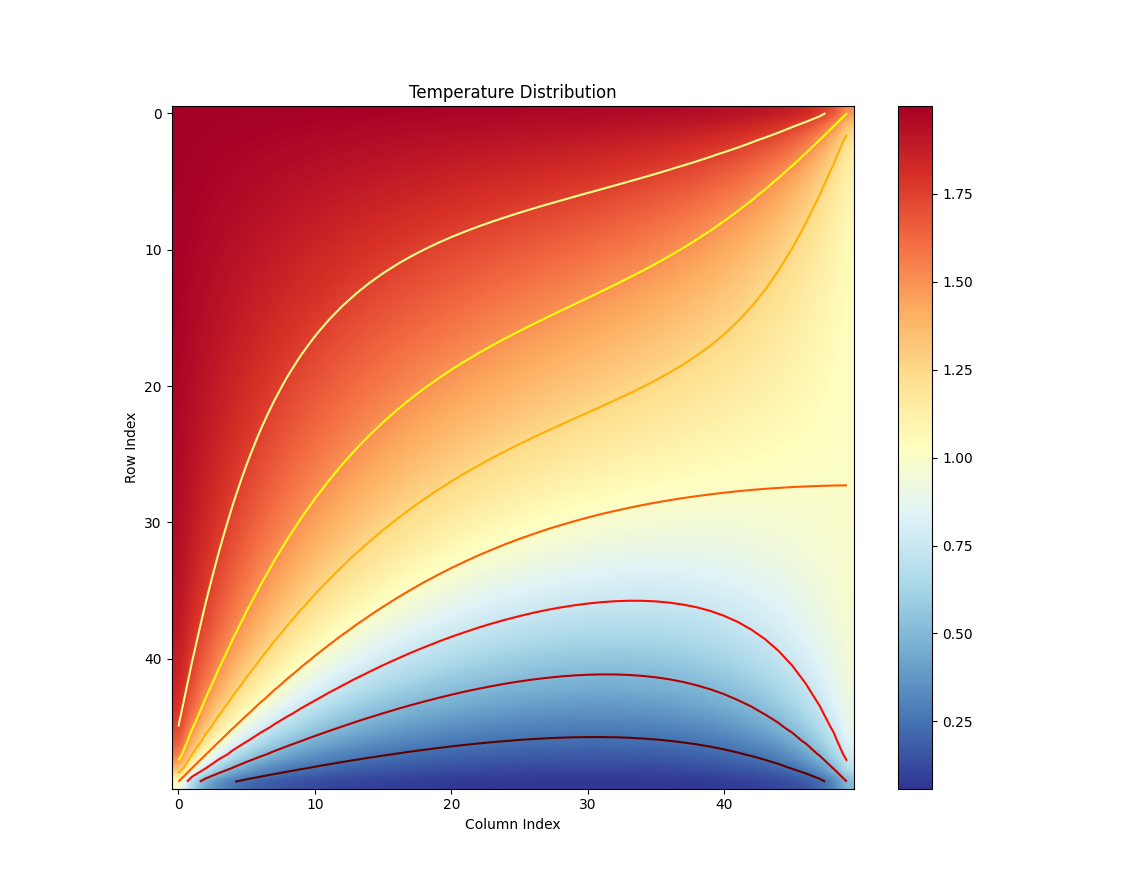
\includegraphics[width=0.45\linewidth]{figures/Figure_1.png}
    \caption{Boundaries $T_{\text{left}}=2, T_{\text{up}}=2, T_{\text{right}}=1, T_{\text{down}}=0$}
  \end{figure}
\end{frame}

\begin{frame}{Results: Example 1}
  \begin{figure}
    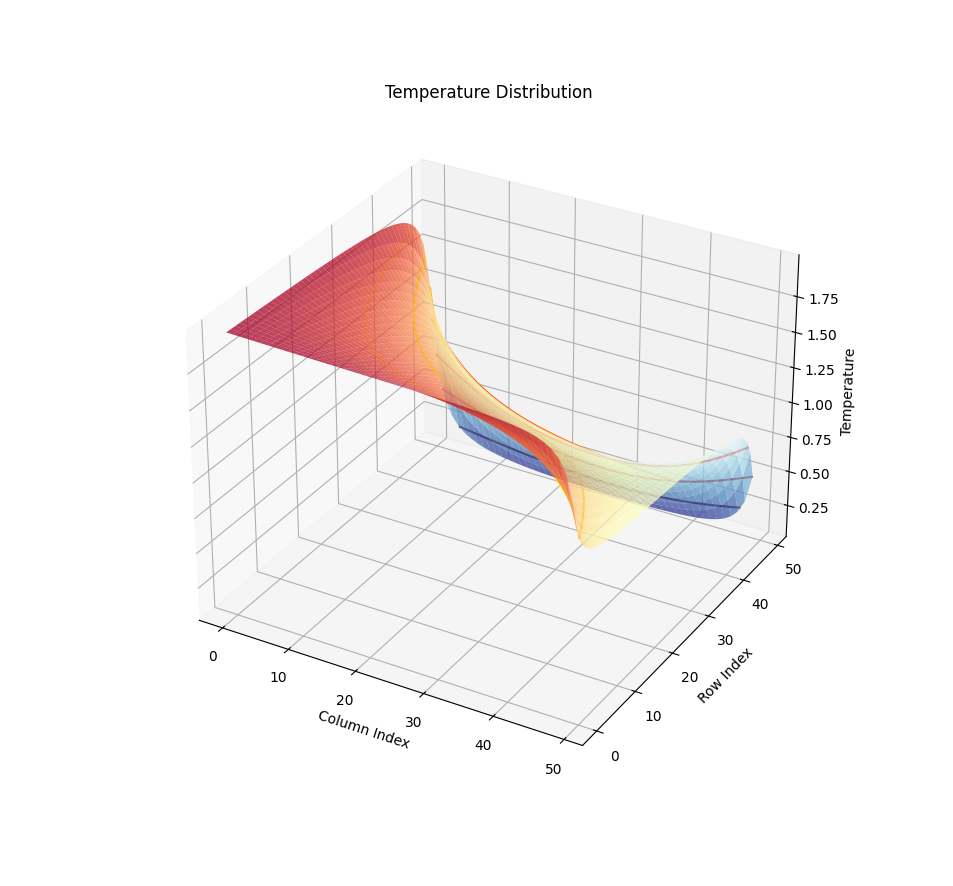
\includegraphics[width=0.4\linewidth]{figures/Figure_2.png}
    \caption{Boundaries $T_{\text{left}}=2, T_{\text{up}}=2, T_{\text{right}}=1, T_{\text{down}}=0$}
  \end{figure}
\end{frame}

\begin{frame}{Results: Example 2}
  \begin{figure}
    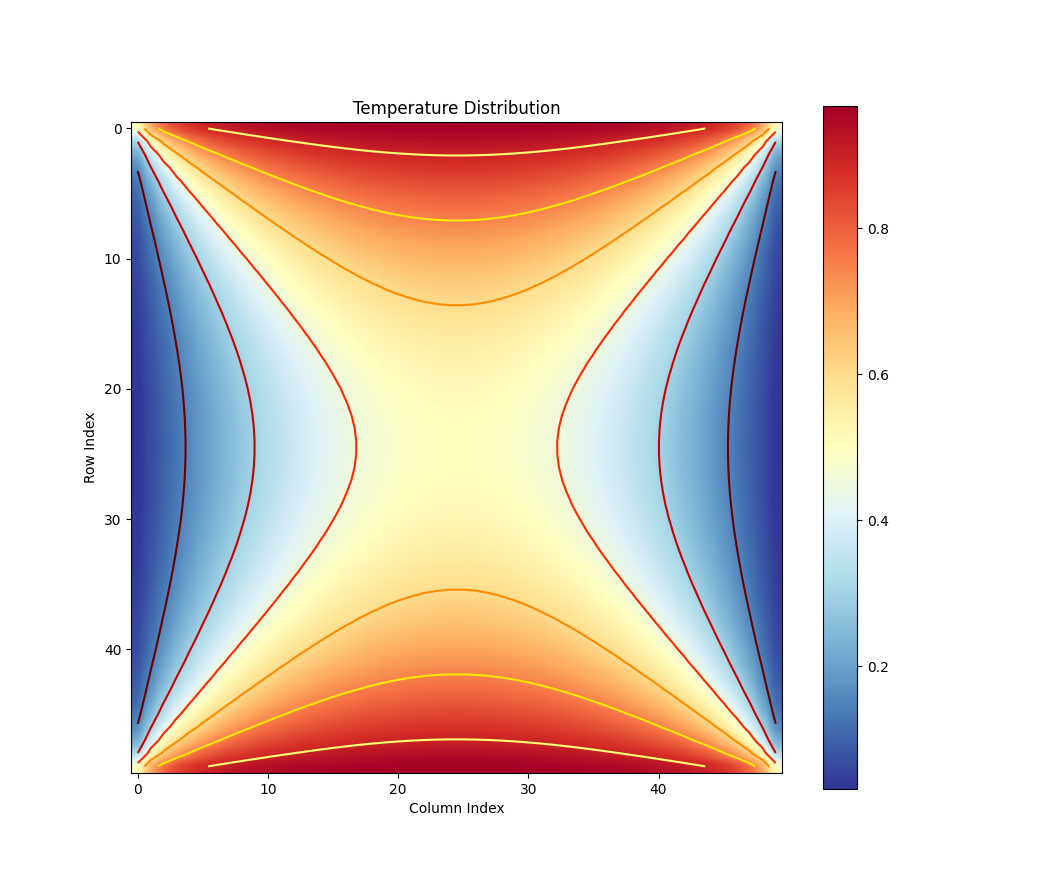
\includegraphics[width=0.45\linewidth]{figures/Figure_3.png}
    \caption{Boundaries $T_{\text{left}}=0, T_{\text{up}}=1, T_{\text{right}}=0, T_{\text{down}}=1$}
  \end{figure}
\end{frame}

\begin{frame}{Results: Example 2}
  \begin{figure}
    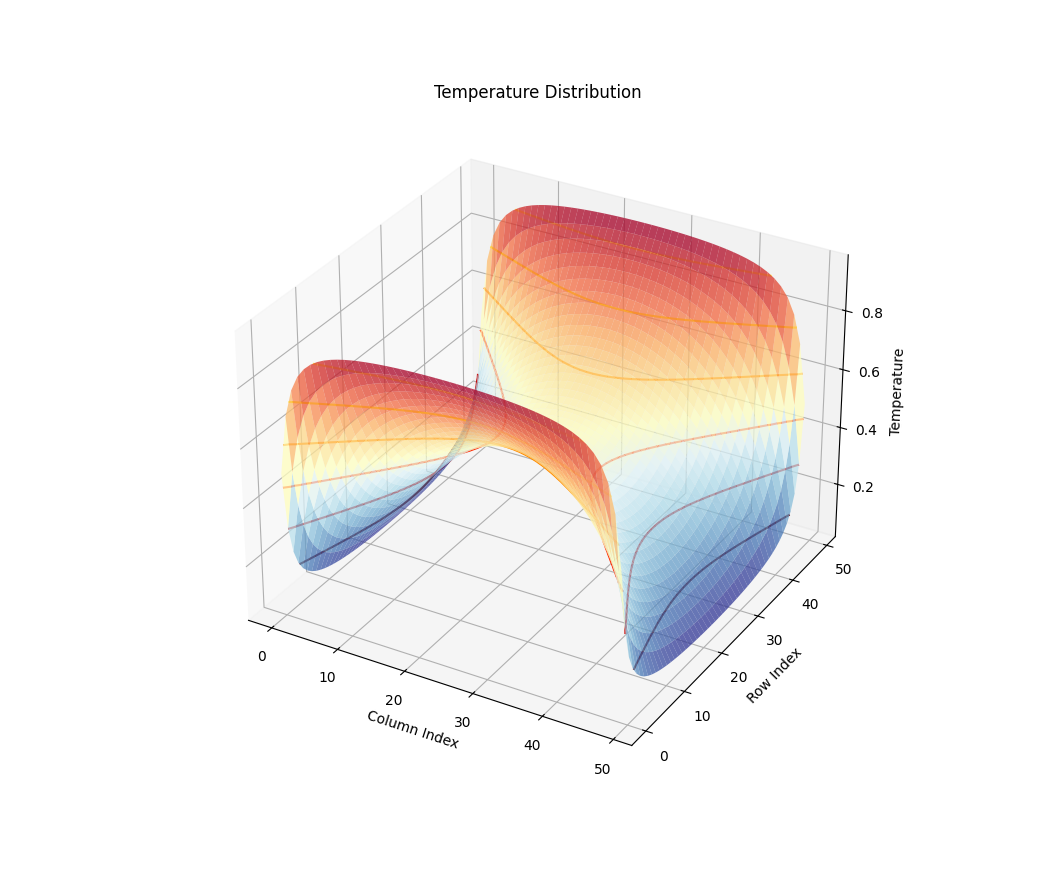
\includegraphics[width=0.45\linewidth]{figures/Figure_4.png}
    \caption{Boundaries $T_{\text{left}}=0, T_{\text{up}}=1, T_{\text{right}}=0, T_{\text{down}}=1$}
  \end{figure}
\end{frame}

% Include more result slides as needed...

\section{Conclusion}

\begin{frame}{Conclusion}
  \begin{itemize}
    \item Linear algebra techniques for solving heat distribution problems.
    \item Insights gained from numerical solutions.
    \item Future work: Extend to more complex geometries.
  \end{itemize}
\end{frame}

\begin{frame}
  \section{Complementary Resources}
  \begin{itemize}
    \item Code Repository: \url{https://github.com/salastro/etd-la}
    \item Iterations Video: \url{https://youtu.be/Zn6hnecikcc}
  \end{itemize}
\end{frame}

\begin{frame}
  \printbibliography
\end{frame}

\end{document}

